%
% ellintegral.tex
%
% (c) 2021 Prof Dr Andreas Müller, OST Ostschweizer Fachhochschule
%
\section{Elliptische Integrale
\label{buch:elliptisch:section:integral}}
\rhead{Elliptisches Integral}
Bei der Berechnung des Ellipsenbogens in 
Abschnitt~\ref{buch:geometrie:subsection:hyperbeln-und-ellipsen}
sind wir auf ein Integral gestossen, welches sich nicht in geschlossener
Form ausdrücken liess.
Um solche Integrale in den Griff zu bekommen, ist es nötig, sie als
neue spezielle Funktionen zu definieren.

\subsection{Definition
\label{buch:elliptisch:subsection:definition}}
Ein {\em elliptisches Integral} ist ein Integral der Form
\index{elliptishes Integral}%
\index{Integral, elliptisch}%
\begin{equation}
\int R\left( x, \sqrt{p(x)}\right)\,dx
\label{buch:elliptisch:def:allgemein}
\end{equation}
wobei $R(x,y)$ eine rationale Funktion von zwei Variablen ist und
$p(x)$ ein Polynom dritten oder vierten Grades.
Hätte $p(x)$ ein mehrfache Nullstelle $x_0$, müsste es durch $(x-x_0)^2$
teilbar sein, man könnte also einen Faktor $(x-x_0)$ aus der
Wurzel im Integraneden von \eqref{buch:elliptisch:def:allgemein}
ausklammern und damit das Integral in eine Form bringen, wo $p(x)$
höchstens zweiten Grades ist.
Solche Integrale lassen sich meistens mit trigonometrischen Substitutionen
berechnen.
Wir verlangen daher, dass $p(x)$ keine mehrfachen Nullstellen hat.

Man kann zeigen, dass sich elliptische Integrale in Summen von
elementaren Funktionen und speziellen elliptischen Integralen 
der folgenden Form überführen lassen
\cite[Abschnitt 164, p.~506]{buch:smirnov32}.

\begin{definition}
\label{buch:elliptisch:def:integrale123}
Die elliptischen Integrale erster, zweiter und dritter Art sind die
Integrale
\[
\begin{aligned}
\text{1.~Art:}&&&
\int \frac{dx}{\sqrt{(1-x^2)(1-k^2x^2)}}
\\
\text{2.~Art:}&&&
\int \sqrt{\frac{1-k^2x^2}{1-x^2}}\,dx
\\
\text{3.~Art:}&&&
\int \frac{dx}{(1-nx^2)\sqrt{(1-x^2)(1-k^2x^2)}}
\end{aligned}
\]
mit $0<k<1$.
Es ist auch üblich, den Parameter $m=k^2$ zu verwenden.
\end{definition}

Wie gesagt lassen sich für diese unbestimmten Integrale keine 
geschlossenen Formen finden.
Es bleibt uns daher nichts anderes übrig, als die Integralgrenzen
festzulegen und damit eine Stammfunktion auszuwählen.

%
% Elliptisches Integral
%
\subsection{Vollständige elliptische Integrale
\label{buch:elliptisch:subsection:vollstaendig}}
In diesem Abschnitt legen wir beide Integrationsgrenzen fest und
untersuchen die entstehenenden Funktionen von den Parametern
$k$ und $n$.

\subsubsection{Definition der vollständigen elliptischen Integrale}
Da der Nenner in allen drei elliptischen Integralen eine Nullstelle
bei $\pm1$ hat, kann das Integral nur von $0$ bis $1$ erstreckt werden.

\begin{definition}
\label{buch:elliptisch:def:vollstintegrale123}
Die vollständigen elliptischen Integrale erster, zweiter und dritter
Art sind
\[
\begin{aligned}
\text{1.~Art:}&&
K(k)&=\int_0^1 \frac{dt}{\sqrt{(1-t^2)(1-k^2t^2)}} \\
\text{2.~Art:}&&
E(k)&=\int_0^1 \sqrt{\frac{1-k^2t^2}{1-t^2}}\,dt \\
\text{3.~Art:}&&
\Pi(n, k)&=\int_0^1\frac{dt}{(1-nt^2)\sqrt{(1-t^2)(1-k^2t^2)}} 
\end{aligned}
\]
mit $0<k<1$.
\end{definition}

Die Funktionen hängen stetig von $k$ ab.
Die Nullstellen des Faktors $1-k^2x^2$ liegen ausserhalb des
Integrationsintervalls und spielen daher keine Rolle.
Die Werte von $K(k)$ und $E(k)$ für $k=0$ können direkt berechnet
werden:
\begin{align*}
K(0)
=
E(0)
&=
\int_0^1 \frac{dt}{\sqrt{1-t^2}}=\frac{\pi}2.
\end{align*}
Das Integral $\Pi(n,0)$ ist etwas komplizierter.

Für $k\to 1$ ist $E(k)=1$, die Integrale $K(1)$ und $\Pi(n,1)$
sind dagegen divergent.

\subsubsection{Jacobi- und Legendre-Normalform}
Die Integrationsvariable $t$ der vollständigen elliptischen Integrale
kann durch die Substitution $t=\sin\varphi$ durch die Variable
$\varphi$ und das Integral über das Intervall $[0,1]$ durch ein
Integral über das Intervall $[0,\frac{\pi}2]$ ersetzt werden.
Mit
\[
\frac{dt}{d\varphi} = \cos\varphi = \sqrt{1-\sin^2\varphi}
\]
können die Funktionen $K(k)$, $E(k)$ und $\Pi(n,k)$ auch als
\begin{align*}
K(k)
&=
\int_0^{\frac{\pi}2}
\frac{
\sqrt{1-\sin^2\varphi}\,d\varphi
}{
\sqrt{(1-\sin^2\varphi)(1-k^2\sin^2\varphi)}
}
=
\int_0^{\frac{\pi}2}
\frac{d\varphi}{\sqrt{1-k^2\sin^2\varphi}}
\\
E(k)
&=
\int_0^{\frac{\pi}2}
\sqrt{\frac{1-k^2\sin^2\varphi}{1-\sin^2\varphi}}\sqrt{1-\sin^2\varphi}\,d\varphi
=
\int_0^{\frac{\pi}2}
\sqrt{1-k^2\sin^2\varphi}\,d\varphi
\\
\Pi(n,k)
&=
\int_0^{\frac{\pi}2}
\frac{
\sqrt{1-\sin^2\varphi}\,d\varphi
}{
(1-n\sin^2\varphi)\sqrt{(1-\sin^2\varphi)(1-k^2\sin^2\varphi)}
}
=
\int_0^{\frac{\pi}2}
\frac{
d\varphi
}{
(1-n\sin^2\varphi)\sqrt{1-k^2\sin^2\varphi}
}
\end{align*}
Diese Form wird auch die {\em Legendre-Normalform} der vollständigen 
\index{Legendre-Normalform}%
elliptischen Integrale genannt, während die Form von
Definition~\ref{buch:elliptisch:def:vollstintegrale123}
die {\em Jacobi-Normalform} heisst.
\index{Jacobi-Normalform}%

\subsubsection{Umfang einer Ellipse}
\begin{figure}
\centering
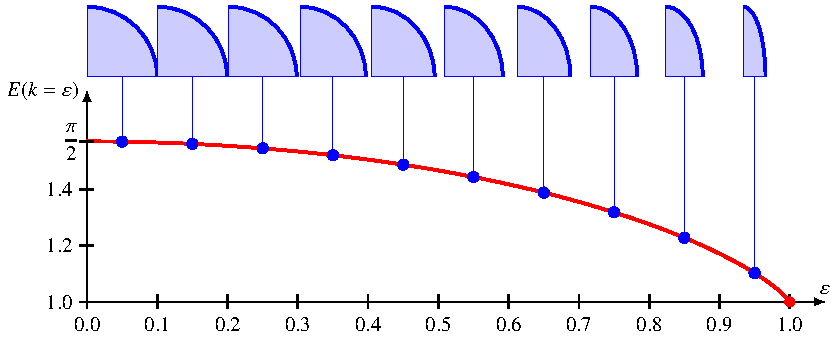
\includegraphics{chapters/110-elliptisch/images/ellipsenumfang.pdf}
\caption{Bogenlänge eines Viertels einer Ellipse mit Exzentrizität
$\varepsilon$.
\label{buch:elliptisch:fig:ellipsenumfang}}
\end{figure}
Wir zeigen, wie sich die Berechnung des Umfangs $U$ einer Ellipse
mit Halbachsen $a$ und $b$, $a\le b$, auf ein volltändiges elliptisches
Integral zurückführen lässt.
Der Fall $a>b$ kann behandelt werden, indem die $x$- und $y$-Koordinaten
vertauscht werden.

Die Parametrisierung
\[
t\mapsto \begin{pmatrix}a\cos t\\ b\sin t\end{pmatrix}
\]
einer Ellipse führt auf das Integral
\begin{align*}
U
&=
\int_0^{2\pi} \sqrt{a^2\sin^2t + b^2\cos^2 t}\,dt
\notag
\\
&=
4\int_0^{\frac{\pi}2}
\sqrt{a^2\sin^2t + b^2(1-\sin^2 t)}
\,dt
\notag
\\
&=
4b \int_0^{\frac{\pi}2} \sqrt{1-(b^2-a^2)/b^2\cdot \sin^2t}\,dt
\label{buch:elliptisch:eqn:umfangellipse}
\end{align*}
für den Umfang der Ellipse.
Bei einem Kreis ist $a=b$ und der zweite Term unter der Wurzel fällt weg,
der Umfang wird $4b\frac{\pi}2=2\pi b$.
Die Differenz $e^2=b^2-a^2$ ist die {\em lineare Exzentrizität} der Ellipse,
\index{lineare Exzentrizität}%
der Quotient $e/b$ wird die {\em numerische Exzentrizität} der Ellipse
genannt.
Insbesondere ist $k = \varepsilon$.

Das Integral~\eqref{buch:elliptisch:eqn:umfangellipse} erhält jetzt die
Form
\[
U
=
4b\int_0^{\frac{\pi}2} \sqrt{1-k^2\sin^2t}\,dt
\]
und ist damit als elliptisches Integral zweiter Art erkannt.
Für den Umfang der Ellipse finden wir damit die Formel
\[
U
=
4b E(k)
=
4b E(\varepsilon).
\]
Das vollständige elliptische Integral zweiter Art $E(\varepsilon)$
liefert also genau den Umfang der eines Viertels Ellipse mit
numerischer Exzentrizität $\varepsilon$ und kleiner Halbachse $1$.

\subsubsection{Komplementäre Integrale}
XXX Komplementäre Integrale \\

\subsubsection{Ableitung}
XXX Ableitung \\
XXX Stammfunktion \\

\subsection{Unvollständige elliptische Integrale}
XXX Vollständige und Unvollständige Integrale \\
XXX Additionstheoreme \\
XXX Parameterkonventionen \\

\subsection{Potenzreihe}
XXX Potenzreihen \\
XXX Als hypergeometrische Funktionen \\


